% \chapter{特殊环境与浮动体}
% \label{chp:float}

% 事实上我们本该假设所有使用本 \LaTeX 论文模板的人都具备了相当的 \LaTeX 使用经验和知识,如果这样那么本章所介绍的内容是不言自明的。但是也存在很多初次接触 \LaTeX 的研究生朋友,因为各种不同的原因而尝试使用 \LaTeX 进行论文排版。因此我们认为还是有必要对这些 \LaTeX 中的基本元素进行反复地强调,以避免我们的个别开发者的邮箱和GitHub Issues被投诉和问询填满。如果你是一个 \LaTeX 老手,你可以直接跳过本章而不用担心漏过任何重要内容。

% \section{图片}

% \subsection{插入图片}
% 在 \LaTeX 文档中插入图片,你需要如下的代码:

% \begin{tcolorbox}
% \begin{lstlisting}[language=TeX]
% \begin{figure}[htbp]
%   \centering
%   \includegraphics[width=.3\linewidth]{figures/content/4_1}
%   \caption{插入图片示例}
%   \label{fig:4_1}
% \end{figure}
% \end{lstlisting}
% \end{tcolorbox}

% \noindent 上面的代码会插入如下效果的图片:

% \begin{figure}[htbp]
%   \centering
%   \includegraphics[width=.3\linewidth]{figures/content/4_1}
%   \caption{插入图片示例}
%   \label{fig:4_1}
% \end{figure}

% \subsection{浮动体环境与位置标识符}

% \begin{tcolorbox}
% \begin{lstlisting}[language=TeX]
% \begin{figure}[htbp]
% \end{figure}
% \end{lstlisting}
% \end{tcolorbox}

% \noindent 声明了一个图片浮动体环境。浮动体是 \LaTeX 中的一种特殊容器,用于容纳占据篇幅较大但不方便分页的内容,如图片或表格。方括号中的字母是浮动体位置标识符,用于向 \LaTeX 编译引擎提出位置建议。常见的位置标识符有以下4种:

% \begin{itemize}
%   \setlength{\itemsep}{1.5pt}
%   \setlength{\parsep}{1.5pt}
%   \setlength{\parskip}{1.5pt}
%   \item {\codefont h}:表示here。\LaTeX 编译引擎在面对用{\codefont h}标识的浮动体时会首先尝试在声明位置插入浮动体;
%   \item {\codefont t}:表示top。\LaTeX 编译引擎会尝试在当页顶部安置浮动体;
%   \item {\codefont b}:表示bottom。\LaTeX 编译引擎会尝试在当页底部安置浮动体;
%   \item {\codefont p}:表示float page。\LaTeX 编译引擎会尝试为该浮动体分页并使其占据全页。
% \end{itemize}
% 你可以使用多个位置标识符并将其自由组合,你指定的顺序代表你向 \LaTeX 编译引擎所推荐的优先级。需要说明的是,编译引擎并不保证会按照你所指定的位置优先级安置浮动体,而是会根据浮动体大小、其在页面中的位置、文字的相对分布等多种因素决定浮动体的位置。因此在论文写作过程中,我们不建议你使用如“下图”,“上表”等使用方位来指代特定图片或表格的表述,因为你所插入的图片或表格很有可能并不会被编译到你想要它出现的位置。当然,你也可以在标识符前加上 !号来表示强制位置,如{\codefont !h}。但是我们不推荐这样做,因为这可能会造成很多你意想不到的后果。

% \subsection{图片的大小与路径}

% \begin{tcolorbox}
% \begin{lstlisting}[language=TeX]
% \centering
% \includegraphics[width=.5\linewidth]{figures/content/4_1}
% \end{lstlisting}
% \end{tcolorbox}

% {\codefont centering}表示浮动体在控制范围内居中。{\codefont includegraphics}语句向编译引擎指定你所想要引入的图片的大小与保存路径。在该命令之后跟随的方括号中,你可以指定图片的长或宽。默认情况下 \LaTeX 会锁定图片的长宽比例,因此你只需要指定长宽中的一个即可。后面的大括号用于填写图片的路径,你可以使用主文件main.tex的相对路径来表示。我们在模板根目录下设置了一个名为figures的目录用于存放图片,我们建议你把论文需要的所有图片放置于该目录下的content文件夹中以便查找和管理。

% \subsection{图片的标题与标签}

% \begin{tcolorbox}
% \begin{lstlisting}[language=TeX]
% \caption{插入图片示例}
% \label{fig:4_1}
% \end{lstlisting}
% \end{tcolorbox}

% {\codefont caption}用于指定图片的标题。{\codefont label}用于给图片添加标签,便于你在文本中引用该图片。对于上面的图片,如果我们想要在论文中引述其内容,可以采用如下方法:

% \begin{tcolorbox}
% \begin{lstlisting}[language=TeX]
% 图\ref{fig:4_1}是东南大学的校徽,它的设计中蕴含着多种寓意。
% \end{lstlisting}
% \end{tcolorbox}

% \noindent 上述文本在编译后会呈现这样的效果:

% 图\ref{fig:4_1}是东南大学的校徽,它的设计中蕴含着多种寓意。

% \subsection{图片的并排}

% 很多时候,你可能会想要将两张图片并排放置以节省排版空间。我们支持并鼓励你这样做。你只需要引入如下的代码:

% \begin{tcolorbox}
% \begin{lstlisting}[language=TeX]
% \begin{figure}[htbp]
%   \centering
%     \begin{minipage}[t]{0.48\textwidth}
%       \centering
%       \includegraphics[width=6cm]{figures/content/4_2}
%       \caption{GitHub}
%       \label{fig:4_2}
%     \end{minipage}
%     \begin{minipage}[t]{0.48\textwidth}
%       \centering
%       \includegraphics[width=8cm]{figures/content/4_3}
%       \caption{NPM}
%       \label{fig:4_3}
%     \end{minipage}
% \end{figure}
% \end{lstlisting}
% \end{tcolorbox}

% \noindent 编译后的效果是这样的:

% \begin{figure}[htbp]
%   \centering
%     \begin{minipage}[t]{0.48\textwidth}
%       \centering
%       \includegraphics[width=4cm]{figures/content/4_2}
%       \caption{GitHub}
%       \label{fig:4_2}
%     \end{minipage}
%     \begin{minipage}[t]{0.48\textwidth}
%       \centering
%       \includegraphics[width=3cm]{figures/content/4_3}
%       \caption{npm}
%       \label{fig:4_3}
%     \end{minipage}
% \end{figure}

% 注意,在上述代码中,我们定义了一个{\codefont figure}浮动体环境,并在其中用两个:

% \begin{tcolorbox}
% \begin{lstlisting}[language=TeX]
% \begin{minipage}[t]{0.48\textwidth}
% \end{minipage}
% \end{lstlisting}
% \end{tcolorbox}

% \noindent 包裹了两张图片的声明。和单个图片类似,你也可以指定{\codefont minipage}相对浮动体的位置和大小。编译引擎将根据你{\codefont minipage}的大小调整在一行显示的图片数量。需要注意的是,在两个{\codefont minipage}声明之间请勿空行,因为 \LaTeX 编译引擎会将空行视作换行请求而错误地将你的两张图片上下放置。

% \subsection{子图}

% 和图片并排类似,子图也用于提供在水平方向上组织浮动体的功能。和图片的简单并排不同的是,子图功能一般用于表达同一主题下内容相近或有对比意义的图片或其他浮动体。对于子图功能,你需要引入如下代码:

% \begin{tcolorbox}
% \begin{lstlisting}[language=TeX]
% \begin{figure}[htbp]
%   \centering
%   \subfloat[彩色标志]{\includegraphics[width=.38\textwidth]{figures/content/4_4}}
%   \quad\quad
%   \subfloat[单色标志]{\includegraphics[width=.38\textwidth]{figures/content/4_5}}
%   \caption{东南大学校徽的视觉设计}
%   \label{fig:4_4}
% \end{figure}
% \end{lstlisting}
% \end{tcolorbox}

% \noindent 编译后呈现如下效果:

% \begin{figure}[htbp]
%   \centering
%   \subfloat[彩色标志]{\includegraphics[width=.38\textwidth]{figures/content/4_4}}
%   \quad\quad
%   \subfloat[单色标志]{\includegraphics[width=.38\textwidth]{figures/content/4_5}}
%   \caption{东南大学校徽的视觉设计}
%   \label{fig:4_4}
% \end{figure}

% \noindent {\codefont subfloat}命令指定了图片的子图单元,你可以在命令后的方括号中指定子图的名称,并在随后的大括号中声明子图的版式和索引路径。

% \section{表格}

% \subsection{插入表格}

% 在论文中插入表格的方法与图片类似,示例代码如下:

% \begin{tcolorbox}
% \begin{lstlisting}[language=TeX]
% \begin{table}[htbp]
% \centering
% \caption{东南大学院系列表}
% \label{tab:4_1}
% \begin{tabular}{cll}
% \toprule
% 院系编号&\multicolumn{1}{c}{院系名称}&\multicolumn{1}{c}{院系英文译名}\\
% \midrule
% 01  & 建筑学院      & School of Architecture  \\
% 02  & 机械工程学院    & School of Mechanical Engineering \\
% 03  & 能源与环境学院   & School of Energy and Environment \\
% 04  & 信息科学与工程学院 & School of Information Science and Engineering \\
% 05  & 土木工程学院    & School of Civil Engineering \\
% \bottomrule
% \end{tabular}
% \end{table}
% \end{lstlisting}
% \end{tcolorbox}

% \noindent 编译后的效果如表 \ref{tab:4_1} 所示。

% \begin{table}[htbp]
% \centering
% \caption{东南大学院系列表}
% \label{tab:4_1}
% \begin{tabular}{cll}
% \toprule
% 院系编号 & \multicolumn{1}{c}{院系名称}       & \multicolumn{1}{c}{院系英文译名 }     \\
% \midrule
% 01                       & 建筑学院      & School of Architecture                        \\
% 02                       & 机械工程学院    & School of Mechanical Engineering              \\
% 03                       & 能源与环境学院   & School of Energy and Environment              \\
% 04                       & 信息科学与工程学院 & School of Information Science and Engineering \\
% 05                       & 土木工程学院    & School of Civil Engineering \\
% \bottomrule
% \end{tabular}
% \end{table}

% \noindent 想要定义一个表格,首先需要声明浮动体环境:

% \begin{tcolorbox}
% \begin{lstlisting}[language=TeX]
% \begin{table}[htbp]
%   \centering
%   \caption{东南大学院系表}
%   \label{tab:4_1}
% \end{table}
% \end{lstlisting}
% \end{tcolorbox}

% \noindent 在声明表格浮动体时,你也可以指定该表格的标题和标签,这与图片的声明类似。需要提醒的是,根据《东南大学研究生学位论文格式规定》\cite{seugs2015rule}第一条第五款第六则的要求,表格的标题应该位于表格的上方,而图片的标题应该出现在图片的下方。

% 表格的具体内容在需要在浮动体中用{\codefont tabular}环境声明:

% \begin{tcolorbox}
% \begin{lstlisting}[language=TeX]
% \begin{tabular}{cll}
%   \toprule
%   院系编号&\multicolumn{1}{c}{院系名称}&\multicolumn{1}{c}{院系英文译名}\\
%   \midrule
%   01  & 建筑学院      & School of Architecture  \\
%   02  & 机械工程学院    & School of Mechanical Engineering \\
%   03  & 能源与环境学院   & School of Energy and Environment \\
%   04  & 信息科学与工程学院 & School of Information Science and Engineering \\
%   05  & 土木工程学院    & School of Civil Engineering \\
%   \bottomrule
% \end{tabular}
% \end{lstlisting}
% \end{tcolorbox}

% \noindent {\codefont tabular}声明后面紧跟着的是表格的纵向对其标准,比如我们的表格有3列,就需要使用3个字母分别指定这3列的对齐准则。你可以使用{\codefont l}表示左对齐,使用{\codefont r}表示右对齐,而使用{\codefont c}表示居中。下面你就可以以行为单位添加表格的内容,行与行间用两条反斜杠隔开,而行中的不同列间使用符号\&隔开。

% 需要特别注意的是,学术论文一般要求所有表格采用三线表形式。对于三线表,其列间不允许存在竖分割线,而行间仅在表顶、表头与表身、表尾处用三条横线确定表格的结构。因此在表格绘制时,你需要手动指定三线的位置,并在相应的行间添加下面三条指令,分别指代顶线、中间线和尾线:

% \begin{tcolorbox}
% \begin{lstlisting}[language=TeX]
% \toprule
% \midrule
% \bottomrule
% \end{lstlisting}
% \end{tcolorbox}

% 事实上,在 \LaTeX 文本中插入表格确实需要付出很大的精力对表格的内容和样式进行调整,这也是很多初学者诟病 \LaTeX 的原因之一。为了方便你设计表格,我们向你推荐\href{http://www.tablesgenerator.com/}{一个网站},该网站能够使用图形化界面创建表格,然后自动生成对应的 \LaTeX 代码。你只需要把代码复制到你的文档中,并稍加调整与修正即可。

% \section{算法}

% 一些理学和工学专业的研究可能需要在论文中插入为代码或算法,本模板同样支持这一功能。示例代码如下:

% \begin{tcolorbox}
% \begin{lstlisting}[language=TeX]
% \begin{algorithm}
% \caption{辗转相除法}
% \label{alg:4_1}
% \begin{algorithmic}
% \Require 一个整数$m$
% \Require 另一个整数$n$
% \Ensure $m$和$n$的最大公约数$r$
% \While {$n > 0$}
%     \State $t \leftarrow m ~ mod ~ n$
%     \State $m \leftarrow n$
%     \State $n \leftarrow t$
% \EndWhile
% \State $r \leftarrow t$
% \end{algorithmic}
% \end{algorithm}
% \end{lstlisting}
% \end{tcolorbox}

% \noindent 上述代码的编译结果如算法 \ref{alg:4_1} 所示。

% \begin{algorithm}
% \caption{辗转相除法}
% \label{alg:4_1}
% \begin{algorithmic}
% \Require 一个整数$m$
% \Require 另一个整数$n$
% \Ensure $m$和$n$的最大公约数$r$
% \While {$n > 0$}
%     \State $t \leftarrow m ~ mod ~ n$
%     \State $m \leftarrow n$
%     \State $n \leftarrow t$
% \EndWhile
% \State $r \leftarrow t$
% \end{algorithmic}
% \end{algorithm}

% 和图片和表格类似,声明算法之前你首先要声明用于安放算法伪代码的浮动体:

% \begin{tcolorbox}
% \begin{lstlisting}[language=TeX]
% \begin{algorithm}
%   \caption{辗转相除法}
%   \label{alg:4_1}
% \end{algorithm}
% \end{lstlisting}
% \end{tcolorbox}

% \noindent 随后使用{\codefont algorithmic}开始添加你的伪代码的具体内容。在这里由于篇幅所限,我们仅会提示一些{\codefont algorithmic}最简单的用法。对于算法的输入项,你需要使用{\codefont $\backslash$Require}命令指明,而输出项使用{\codefont $\backslash$Ensure}命令。对于声明和赋值语句,请你以{\codefont $\backslash$State}开头,而对于判断、循环语句,应该使用如下的形式表达:

% \begin{tcolorbox}
% \begin{lstlisting}[language=TeX]
% \If \EndIf
% \While \EndWhile
% \For \EndFor
% \end{lstlisting}
% \end{tcolorbox}

% \noindent 请注意,这些语句必须两两配对,否则编译时会出现错误。想要了解更多{\codefont algorithmic}的用法和范例,请自行百度或者参考其官方文档。

% \section{公式环境}

% 很多时候,你的论文可能会涉及公式和逻辑推导,这时你可能需要插入数学公式环境。\LaTeX 中的数学公式分为两种,分别是行内公式和行间公式环境。当你想要在文本叙述中插入数学符号时,你需要的是行内公式。你只需要用两个\$符号包裹你的数学符号即可,就像这样:

% \begin{tcolorbox}
% \begin{lstlisting}[language=TeX]
% 对于$\forall \theta \in \Theta$,如果有$\theta$使得...
% \end{lstlisting}
% \end{tcolorbox}

% \noindent 编译后的结果是这个样子的:

% 对于$\forall \theta \in \Theta$,如果有$\alpha$使得...

% 但是当你想要表达数学逻辑的推导或者方程的计算时,你可能需要整块行间的区域进行系统性地阐述,这时你需要使用行间公式环境。就像这样:

% \begin{tcolorbox}
% \begin{lstlisting}[language=TeX]
% \begin{equation}
%   \label{eq:4_1}
%   f(x) = \frac{f(x_0)}{0!} + \frac{f'(x_0)}{1!}(x-x_0) + \dots + \frac{f^{(0)}(x_0)}{n!}(x-x_0)^n + R_n(x)
% \end{equation}
% \end{lstlisting}
% \end{tcolorbox}

% \noindent 上述代码编译后将呈现这样的效果:

% \begin{equation}
%   \label{eq:4_1}
%   f(x) = \frac{f(x_0)}{0!} + \frac{f'(x_0)}{1!}(x-x_0) + \dots + \frac{f^{(0)}(x_0)}{n!}(x-x_0)^n + R_n(x)
% \end{equation}

% \noindent 公式 \ref{eq:4_1} 展示了单行行间公式的表达方式。有时候你还可能需要展示多行的公式,并且这些公式还要按照某些方式对齐。这时候你需要在{\codefont equation}环境中再嵌套一个{\codefont aligned}环境。在每行需要对齐的部分,你可以使用{\codefont \&}符号显式地指明,就像这样:

% \begin{tcolorbox}
% \begin{lstlisting}[language=TeX]
% \begin{equation}
%   \label{eq:4_2}
%   \begin{aligned}
%   \int_{-\infty}^{\infty}f(x)dx & = \frac{1}{2\lambda}\int_{-\infty}^{\infty}e^{-\frac{|x-\mu|}{\lambda}}dx \\
%   & = \frac{1}{2}\int_{-\infty}^{\infty}e^{-|t|}dt \\
%   & = 1
%   \end{aligned}
% \end{equation}
% \end{lstlisting}
% \end{tcolorbox}

% \noindent 上述代码编译后将呈现这样的效果:

% \begin{equation}
%   \label{eq:4_2}
%   \begin{aligned}
%   \int_{-\infty}^{\infty}f(x)dx & = \frac{1}{2\lambda}\int_{-\infty}^{\infty}e^{-\frac{|x-\mu|}{\lambda}}dx \\
%   & = \frac{1}{2}\int_{-\infty}^{\infty}e^{-|t|}dt \\
%   & = 1
%   \end{aligned}
% \end{equation}

% 我们只展示了一小部分数学公式的语法,如果你有更复杂的表达需求,请自行百度。

% \section{引用浮动体}

% 我们已经在 \ref{sec:main_body} 节中介绍了正文章节的引用,并在本章展示了对图、表、算法和公式的引用。为了使你在面临大量标签时也能够快速找到你需要引用的内容,同时也为了提升你文档的结构与条理,我们建议你分别用不同的前缀表记不同类型的引用对象,就像这样:

% \begin{tcolorbox}
% \begin{lstlisting}[language=TeX]
% \label{chp:chapter_name}
% \label{sec:section_name}
% \label{subsec:subsection_name}
% \label{fig:figure_name}
% \label{tab:table_name}
% \label{alg:algorithm_name}
% \label{eq:equation_name}
% \end{lstlisting}
% \end{tcolorbox}

% \noindent 你也可以设计你自己的引用标签,上面的示例只是我们的一个建议。很多编辑器在你输入{\codefont ref}时会自动弹出代码提示,自定义标签配合代码提示能够帮助你更快索引到你想要的引用标签。

% \section{代码环境}

% 一些计算机、软件、电子等专业的毕业论文可能需要展示少量代码,本模板同样也提供了代码环境。比如,下面我们展示了一个Java程序:

% \begin{tcolorbox}
% \begin{lstlisting}[language=Java]
% public static void main(String[] args) {
%     System.out.println("你好世界");
% }
% \end{lstlisting}
% \end{tcolorbox}

% 想要实现这样的效果,你只需要将代码包裹在{\codefont lstlisting}环境中。你还可以指定代码所属的语言,这样{\codefont lstlisting}环境就可以为你实现一定程度上的代码高亮。想要查询你所使用的计算机语言是否被{\codefont lstlisting}支持,请直接参阅{\codefont lstlisting}的官方文档。

% \section{术语与符号}

% 你的论文中可能涉及到了大量的符号、英文缩写或术语,你可以在文中对这些符号进行说明,就像这样:

% \begin{tcolorbox}
% \begin{lstlisting}[language=TeX]
% \nomenclature{PDF}{Portable Document Format}
% \end{lstlisting}
% \end{tcolorbox}

% \noindent 你应该在{\codefont nomenclature}命令后的第一对括号中填写术语或符号名称,下一对括号中填写对术语或符号的解释或定义。当论文编译时,这些术语与符号将会被自动列入目录页后的术语与符号表,并按照英文字母序排列。


\chapter{无线信道密钥生成流程}

本章将详细的介绍无线密钥生成系统设计和实现的具体细节,介绍上层应用利用导频信号收发机实现信道探测的过程。% TODO 补完介绍

\section{TDD/FDD系统信道探测系统研究设计}

在上一章节中,本文介绍了如何利用GNURadio设计密钥生成系统所需要的模块搭建导频信号收发机,导频信号收发机使用如图\ref{tranceiver_structure}四个模块完成TDD/FDD系统中信号的发送和接收。

\begin{figure}[htbp]
    \centering
    \includegraphics[width=0.9\textwidth]{images/tranceiver_structure}
    \caption{导频信号收发机}{} 
    \label{tranceiver_structure}
\end{figure}

对于TDD系统来说,Alice与Bob之间的信道探测过程如图\ref{two_tranceiver_structure}所示。对于FDD系统来说,Alice与Bob之间的信道探测过程如图\ref{two_tranceiver_structure_fdd}所示。TDD和FDD系统中不同的地方在于,TDD系统的通信双方在同一个频点上发射和接收导频信号,而FDD系统的通信双方在不同的频点上发射和接收导频信号。

% \begin{figure}[htbp]
%   \centering
%   \begin{minipage}[t]{0.5\textwidth}
%   \centering
%   \includegraphics[width=6cm]{images/two_tranceiver_structure}
%   \caption{TDD系统中的信道探测}{} 
%   \label{two_tranceiver_structure}
%   \end{minipage}
%   \begin{minipage}[t]{0.5\textwidth}
%   \centering
%   \includegraphics[width=6cm]{images/two_tranceiver_structure_fdd}
%   \caption{FDD系统中的信道探测}{} 
%   \label{two_tranceiver_structure_fdd}
%   \end{minipage}
% \end{figure}

\begin{figure}[htbp]
    \centering
    \includegraphics[width=0.6\textwidth]{images/two_tranceiver_structure}
    \caption{TDD系统中的信道探测}{} 
    \label{two_tranceiver_structure}
\end{figure}



TDD系统中,通信双方分Master和Slave端。Slave端的检波模块只有检测到Master端发射的导频信号,才会发射导频信号,因此Slave端的导频信号检测模块和导频序列输出模块之间存在信号事件。FDD系统中,通信双方的地位是对等的,不分主从,Slave发射导频信号是不受Master影响的,因此导频信号检测模块和导频序列输出模块之间也不存在信号事件。

为了实现信号事件,本文使用GNURadio中$gr::basic_block$提供的消息传递接口。在GNURadio中,$gr::basic_block$是所有模块的父类,模块也会区分输入和输出端口。该类提供了消息订阅与通知机制,如果某个模块注册了某个端口,那么当该模块在该端口发布消息时,任何订阅该模块同名端口的模块都会收到该消息并根据消息类型作出不同的响应行为。实际上,当模块在某端口发布消息时,该模块会迭代所有订阅同名端口的模块,并调用成员方法将消息压入到订阅模块的消息队列中去,如图\ref{message_passing}所示。本文实现了导频信号检测模块和导频序列输出模块之间的消息通知,并加入延迟这一参数观察不同延迟时间下信道和密钥生成的结果。

\begin{figure}[htbp]
  \centering
  \includegraphics[width=0.6\textwidth]{images/two_tranceiver_structure_fdd}
  \caption{FDD系统中的信道探测}{} 
  \label{two_tranceiver_structure_fdd}
\end{figure}

\begin{figure}[htbp]
    \centering
    \includegraphics[width=0.6\textwidth]{images/message_passing}
    \caption{消息传递接口}{} 
    \label{message_passing}
\end{figure}

\section{信道估计}

本文使用的导频信号如图\ref{tx_pilot}所示,系统检波得到的导频信号如图\ref{rx_pilot}所示。在密钥生成协议中,通信双方均已得知导频信号的组成部分,因此可以通过已知导频信号和接收导频信号估计得到信道。

\begin{figure}[htbp]
    \centering
    \includegraphics[width=0.9\textwidth]{images/tx_pilot}
    \caption{发射导频信号}{} 
    \label{tx_pilot}
\end{figure}

\begin{figure}[htbp]
    \centering
    \includegraphics[width=0.9\textwidth]{images/rx_pilot}
    \caption{接收导频信号}{} 
    \label{rx_pilot}
\end{figure}

假设某通信方发射的导频信号$P(k)$,则其数据成分依次为表\ref{component_of_pilot}所示。空数据点是为了避免USRP发射导频信号时初始数据点增益较小的可能,首尾两端正弦波用于粗同步,m序列CP前缀是避免干扰,m序列用于精同步和信道估计。

\begin{table}[]
    \centering
    \begin{tabular}{|l|l|}
    \hline
    组成成分 & 长度(复数点个数)\\ \hline
    空数据点 & 2000 \\ \hline
    首端正弦波 & 1504 \\ \hline
    m序列cp前缀 & 129 \\ \hline
    m序列 & $ 4095 = 2^{12} - 1 $ \\ \hline
    OFDM数据 & 1280 \\ \hline
    尾端正弦波 & 1504 \\ \hline
    \end{tabular}
    \caption{导频信号的组成成分
    \label{component_of_pilot}}
\end{table}

\subsection{频偏估计}

由于信道的非线性、收发两端晶振差异、移动环境中的多普勒频移,接收的导频信号需要进一步消除频率偏移。
在接收的导频信号中,可以使用首尾两端的正弦波来进行频偏估计。假设利用正弦波中的$Sine(k)$部分进行频率估计,对于间隔点数$\tau$来说,对载波频偏进行粗估计,有

\begin{align}
    z(\tau) & = \frac{1}{N - \tau} \sum_{i = 1}^{N-\tau} \bar{Sine(i)} \times Sine(i + \tau) \\
    & = \frac{1}{N-\tau} \sum_{i = 1}^{N-\tau} e^{-jwi\epsilon} e^{jw(i+\tau)\epsilon} \\
    & = \frac{1}{N-\tau} \sum_{i = 1}^{N-\tau} e^{jw\tau\epsilon}
\end{align}

本文计算了$L_{\tau} = 5$次粗估计,即$\tau \in \{1,..., L_{\tau}\}$,并求出相位值phase

\begin{equation}
    p(\tau) = \frac{1}{2\pi} tan^{-1} {\frac{Im(z(\tau))}{Re(z(\tau))}}
\end{equation}

并将$p(\tau)$序列通过$\pm \pi$调整成递增或者递减序列$\tilde{p(\tau)}$,并除以对应的间隔点长度$\tau$,得到补偿因子序列为,

\begin{equation}
    \epsilon(\tau) = \tilde{p(\tau)} / \tau
\end{equation}

最终频率补偿因子为$\epsilon(\tau)$的平均值$\bar{\epsilon}$,并通过其方差判断该补偿因子是否误差较大,如果较大则舍弃不用。因为有首尾两段正弦波,通过这两端正弦波分别估计出$\bar{\epsilon}_1$和$\bar{\epsilon}_2$,以及对应的方差$\sigma_1$和$\sigma_2$。如果$\sigma_1$和$\sigma_2$均大于阈值$Threshold_{\sigma}$,则取其平均数作为补偿因子;如果$\sigma_1$和$\sigma_2$均小于阈值$Threshold_\sigma$,则均舍弃不用;如果一大一小,则取其中满足大于阈值的因子作为补偿因子。

另外可以利用两端正弦波一起做频偏估计,即对相隔距离为$\tau_{12}$、长度均为$N$的正弦波$Sine_1$和$Sine_2$综合起来作,

\begin{equation}
    z = \frac{1}{N} \sum_{i=1}^N Sine_1(i) \times \tilde{Sine_2(i)}
\end{equation}

由于,

\begin{equation}
    Sine_2(i) = Sine_1(i - \tau{12})
\end{equation}

则

\begin{align}
    z = & \frac{1}{N} \sum_{i=1}^N e^{-jwi\epsilon} e^{jw(i+\tau_{12})\epsilon} \\
      = & \frac{1}{N} \sum_{i=1}^N e^{jw\tau_{12}\epsilon} \\
\end{align}

\begin{equation}
    p = \frac{1}{2\pi} tan^{-1} \frac{Im(z)}{Re(z)} 
\end{equation}

\begin{equation}
    \epsilon = p / \tau_{12}
\end{equation}


\subsection{信道补偿}

通过频偏估计得到补偿因子$\epsilon$,本文采用频率补偿的方法是直接对原信号补偿,即在离散傅里叶变换进行频率偏移的补偿,则对信号$S(k)$补偿的结果为,

\begin{equation}
    \tilde{S(k)} = S(k) * e^{2\pi \epsilon k}
\end{equation}

\subsection{信道估计}

从频偏补偿之后的导频信号中截取m序列$\tilde{m(k)}$,并和已知原始信号$m(k)$进行信道估计,

\begin{equation}
    h(k) = \sum_{i=1}^{L_m} \tilde{m(i)} \times m( (i + k) mod L_m )
\end{equation}

通过FFT得到频域响应,然后移除直流分量,再滑动平均,最终得到信道估计的结果。

\begin{equation}
    H(k) = MA(FFT(h(k)))
\end{equation}

如图\ref{ma_before_after_res}是平滑前和平滑后的频率响应结果。

% /home/ruiy/store/data/experiment/indoor-no-move-600/alice/2019-04-01-10-48-12/csi 
\begin{figure}[htbp!]
    \centering \includegraphics[width=0.9\textwidth]{images/ma_before_after_res} 
    \caption{平滑前后CSI结果}
    \label{ma_before_after_res}
\end{figure}

\section{特征量化}

对CSI进行降采样一方面可以提高密钥一致率,另一方面可以降低密钥泄露率。降采样之后,再进行归一化处理。本文先将CSI归一化到$[0, 2^L)$的范围内,并四舍五入得到整数值,其中L为整数。再除以$2^{(L - R)}$并向下取整得到最终量化值,其中R为量化阶数。

设CSI序列为$CSI(k)$,则首先归一化,

\begin{equation}
    Norm(k) = Round(\frac{(2^L - 1) CSI(k)}{Max(CSI)}
\end{equation}

再量化,

\begin{equation}
    Quant(k) = \frac{Norm(k)}{2^{(L - R)}}
\end{equation}

其中, $Round(\cdot)$为四舍五入,$Max(\cdot)$为取最大值

再进行格雷编码,减少比特的不一致率,最后再进行8b10b编码使得01比特的分布更加均匀、随机。

本文使用上述方式进行均匀量化,其中$L = 7$,$R = 3$,\ref{quantization_and_csi}所示为某次室外测量过程中,探测得到的CSI和其量化之后的部分结果。图中展示了通信双方Alice和Bob的CSI结果以及量化得到的部分比特流,可以看出Alice和Bob的CSI较为接近且生成的比特流相似,但是窃听者Eve测量得到CSI与合法通信方相差很大并且量化得到的比特流也相差较大。

\begin{figure}[htbp!]
    \centering 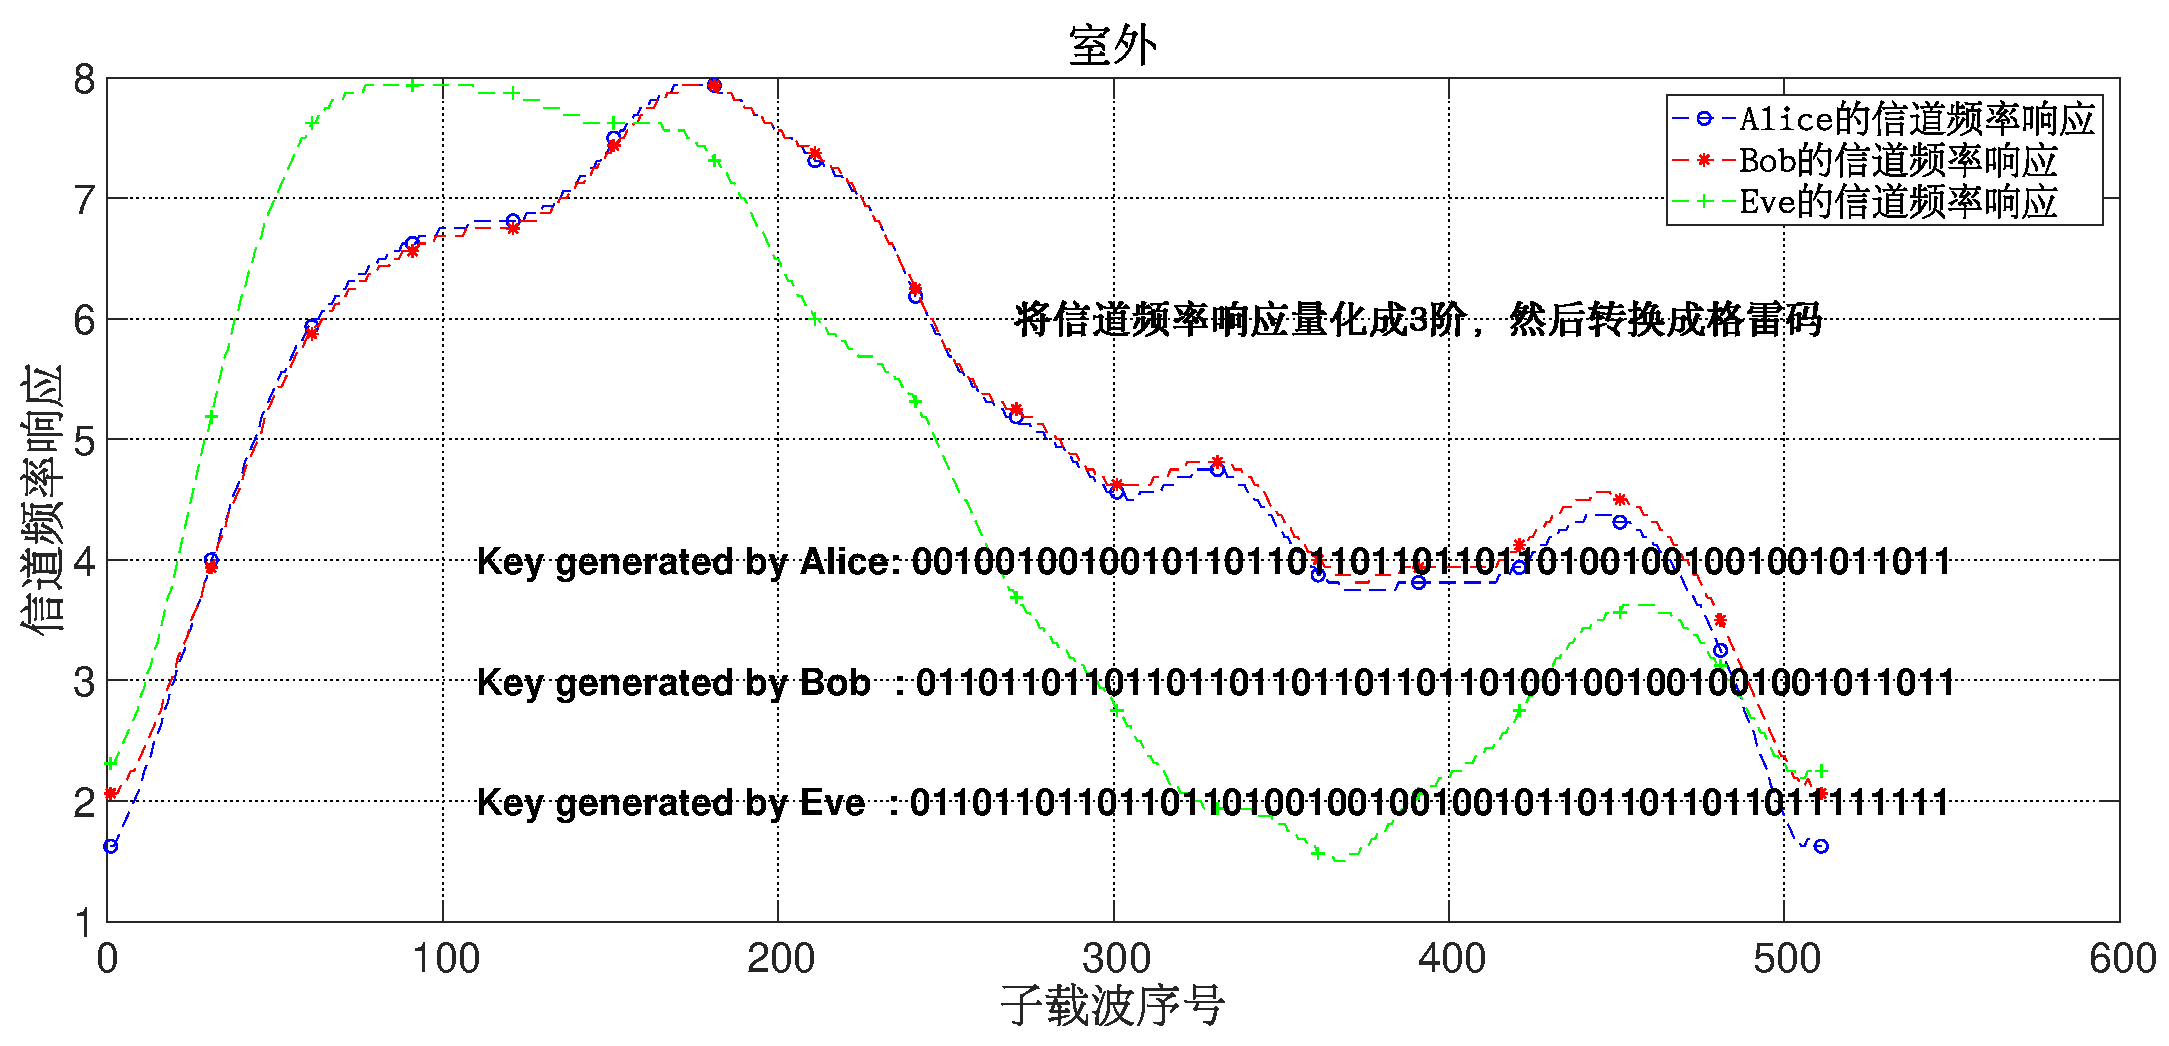
\includegraphics[width=0.9\textwidth]{images/quantization_and_csi} 
    \caption{量化之后的CSI}
    \label{quantization_and_csi}
\end{figure}

\section{信息调和}

在特征量化之后,通信双方需要进一步调和来消除密钥流中不一致的比特。在通信过程中,由于通信系统的上下行特性、硬件指纹、环境噪声等原因,通信双方测量得到的CSI虽然相似,却并不完全一致,进而导致生成密钥比特流中存在不一致的比特。因此需要通信双方结合信息调和来得到完全一直的比特流。本文实现了两种信息调和的方法。

一种是基于CRC校验的信息调和方法,这种方法通过对比特流分组,并对每组生成CRC校验码,通信双方比较每一组的校验码,校验码不一致的组直接舍弃、校验码相同的组保留。该方法的安全性取决于分组的大小,因为调和过程在公共信道进行,所以窃听者可以窃听到调和的信息并根据泄露信息预测出部分密钥的信息。对于本方法来说,由于公共信道上传递的是CRC校验冗余码,因此每组比特数越小,泄露的信息量就越小。

另外一种基于纠错码的信息调和方法,该方法将需要传递的会话密钥进行纠错编码,之后与特征量化步骤中生成的比特流依次异或加密,再通过公共信道发送给对方。对方收到之后同样先和比特流依次进行异或解密,再进行纠错解码,得到会话密钥。在特征量化步骤中,通信双方量化生成的比特流并不一致,该方法实际上将不一致的比特位当做信道过程中的干扰项,并基于纠错码的特点对不一致的比特进行纠错。当错误比特数超过纠错码性能时,接收方就无法正确恢复纠错码。为了接收方可以判断恢复得到的会话密钥的正确性,发送方在调和时会附带会话密钥的摘要,接收方在恢复出会话密钥之后,可以生成新摘要与其对比,便可以判断出是否纠正成功,如果纠错失败,则需要重新开始密钥协商过程。该方法同样存在调和过程中信息泄露的问题,分组过小,那么窃听者可以窃取更多的信息;分组过大,则纠错将会更加困难\cite{李古月2014无线信道的密钥生成方法}。

\subsection{基于CRC校验码的调和方法}

循环冗余校验(cyclic redundancy check, CRC)是一种错误检测方式,用于检测传输数据或者存储数据的意外更改。该方法将数据分块,并根据生成多项式作多项式除法得到校验冗余码。在检查时,会重复计算冗余码是否相同,如果冗余码不匹配,则说明数据被意外更改并进行纠错。

假设某长度为$L$数据块的多项式表示为$M(x)$,$M(x)$中多项式系数表示数据块中的每一位。$G(x)$为$n+1阶$的生成多项式,作为除数,用于生成校验冗余码。将$M(x)$各项同时乘以$x^n$,相当于在二进制字符串后面添加n个0,则$M(x) \cdot x^n$可以表示成,

\begin{equation}
    M(x) \cdot x^n = Q(x) \cdot G(x) - R(x) 
\end{equation}

其中$Q(x)$是除法结果,$G(x)$为除数,$R(x)$即所需校验冗余码。发送方会对每个数据块作相同处理,并将冗余码发送给接收方。接收方同样对数据分组,设相同位置的数据块为$M'(x)$,则检查$M'(x) * x^n + R(x)$是否可以被$G(x)$整除。如果可以整除,那么说明$M'(x)$与$M(x)$一致,那么该组数据块可以保留,否则舍弃不用。接收方以此方式对每组数据块作判断,最后得到校验结果向量$Vec(k)$,并传输给发送方,发送方再以此去除分组中校验不一致的组。

本文使用CRC-12校验,其生成多项式为$x^{12}+x^{11}+x^{3}+x^{2}+x+1$,对应字符串为$1100000001111$或者十六进制表示为$0x80F$。\ref{bitstream_and_crccode}展示了某次测量过程中,Alice和Bob量化之后的比特流按7分组的结果、Alice分组计算得到的CRC冗余码、Bob根据Alice发送过来的冗余码得到的校验结果(1表示匹配,0表示不匹配)。

\begin{figure}[htbp!]
    \centering \includegraphics[width=0.9\textwidth]{images/bitstream_and_crccode} 
    \caption{CRC校验码}
    \label{bitstream_and_crccode}
\end{figure}

\subsection{基于纠错码的调和方法}

本文使用了两种纠错码,Turbo码和BCH码。首先Alice会生成随机数作为密钥,并使用Turbo码或者BCH码进行纠错编码,再异或CSI量化出的密钥比特流。之后将其发送给Bob,Bob将其和比特流异或,再进行纠错解码。除了Turbo和BCH码之外,还有LDPC码等方式。

\subsubsection{Turbo码}

Turbo码于1993年由Claude Berrou等人提出,其实现方式以时间换取逼近香农极限的性能。Turbo码的编码器和解码器如图\ref{turbo_encode}和\ref{turbo_decode}所示。Turbo码的译码算法包括MAP算法、LOG-MAP算法、Max-Log-MAP算法和SOVA算法,本文使用LOG-MAP和SOVA算法来进行译码。另外迭代次数也会影响译码算法,迭代次数越高,对信息比特的估计就越精确,但是迭代次数到达一定数值之后,译码性能改善太小。

\begin{figure}[htbp!]
    \centering \includegraphics[width=0.6\textwidth]{images/turbo_encode} 
    \caption{Turbo编码}
    \label{turbo_encode}
\end{figure}

\begin{figure}[htbp!]
    \centering \includegraphics[width=0.9\textwidth]{images/turbo_decode} 
    \caption{Turbo解码}
    \label{turbo_decode}
\end{figure}


\subsubsection{BCH码}

BCH码(BCH codes、Bose–Chaudhuri–Hocquenghem codes)为取自Bose、Ray-Chaudhuri与Hocquenghem的缩写,是一种循环纠错码,BCH码能灵活地选择码参数,如分组长度和码率,当分组长度为几百或者更少时,BCH码被公认为同样分组长度和码率的编码中最好的码之一。

对于任意的正整数m($m \leq 3 $)和t ($ t < \frac{2^m - 1}{2} $),存在二进制BCH码满足,

则该BCH码可以检测和纠正多达t个随机的误码。设$\alpha$为有限域$GF(2^m)$的本原根。则长度$2^m - 1$、t纠错能力的BCH码的生成多项式$g(x)$是$GF(2)$上根为$\alpha$、${\alpha}^2$、${\alpha}^3$、...、${\alpha}^{2t}$的极小多项式。设$\phi_i(x)$是$\alpha^i$的极小多项式。那么$g(x)$一定是$\phi_1(x)$、$\phi_2(x)$...$\phi_{2t}(x)$最小公倍数。即,

\begin{equation}
    g(x) = LCM\{\phi_1(x), \phi_2(x), ... , \phi_{2t}(x)\}
\end{equation}

如果i是偶数,那么可以表示成乘积形式,

\begin{equation}
    i = i'2^l
\end{equation}

其中$i'$是奇数,并且$l \leq 1$,则$\alpha^i = (\alpha^{i'})^{2^l}$是$\alpha^{i'}$的共轭,因此$\alpha^i$和$\alpha^{i'}$有相同极小多项式,因此,

\begin{equation}
    \phi_i(x) = \phi_{i'}(x)
\end{equation}

因此,$\alpha$的偶数方和$\alpha$的奇数方有相同的极小多项式,故,

\begin{equation}
    g(x) = LCM\{\phi_1(x), \phi_3(x), ... , \phi_{2t-1}(x)\}
\end{equation}

\begin{table}[]
  \centering
  \begin{tabular}{|l|l|l|}
  \hline
  块长度 & $ n = 2^m - 1 $  \\ \hline
  消息比特数 & $ k \leq n - mt $  \\ \hline
  最小距离 & $ d_{min} \leq 2t + 1 $  \\ \hline
  \end{tabular}
  \caption{
  \label{}}
\end{table}

由于$ deg[\phi_i(x)] \leq m $,所以$ deg[g(x)] \leq mt $,所以 $ n -k \leq mt $。这意味着校验位的个数$n - k $最多为$mt$。当$t$非常小时,$n - k $和$mt$十分相近。

当纠错单个误码时,即汉明码。此时$g(x) = \phi_1(x)$并且$t = 1$,因为$\alpha$是$GF(2^m)$域上的本原元素,所以$\phi_1(x)$是阶数m的本原多项式,此时,

\begin{equation}
    \alpha_{2^0}, \alpha_{2^1}, \alpha_{2^2}, ..., \alpha_{2^m} = 1
\end{equation}

所以长度为$2^m - 1$、可以纠错1个误码的BCH码就是汉明码。

\section{隐私放大}

在信道探测阶段和信息调和阶段,所有交互信息对任何第三方都是可见的,这些信息中携带密钥信息,因此需要进一步进行隐私放大。通常使用哈希函数来进行隐私放大,哈希函数的单向性使得窃听者无法从公开信息中分析出密钥信息。常见的哈希函数有MD5、SHA(Secure Hash Algorithm)算法等等。本文使用SHA-2来作隐私放大,Alice和Bob将调和得到的会话密钥分别送入哈希函数,得到512比特的密钥值。